\chapter{Theoretical Background}
\label{chapter:background}
\begin{music}
    \parindent10mm \instrumentnumber{1} \setstaffs1{1} 
    \generalmeter{\meterfrac34} \generalsignature{-1}
    \startextract
		\notes  \en
    \zendextract
\end{music}
\epigraph{\textit{the passion of friendship will soon blossom into a righteous power}}{Bolero of Fire --- Ocarina of Time}

% Convolutional neural networks trained on large databases \cite{mnist2012,imagenet2009} have shaped machine learning research over the past couple of decades. Today they serve as canonical learning material in courses and are often used as initial \textit{vanilla} approaches for data exploration and classification tasks and before creating more bespoke machine learning pipelines. The widespread success of much models created an expectation in the research community that with sufficient data and computational power provided by one of the reigning consumer internet businesses, a data-driven black-box model can be created for any application ranging from quantum mechanics to economics. Convolutional architectures together with language models eventually inspired recurrent architectures and attention models where are the key ingredients in the creation of \textit{Alpha Fold} \cite{Jumper2021HighlyAlphaFold} that takes a substantial step towards solving the protein-folding problem. Biotechnology researchers are eager to apply these methods but face the following obstacles

% \begin{itemize}
%     \item \textbf{Insufficient data} due to strategic experimental designs 
%     \item \textbf{Low extrapolation accuracy} for black box-models
% \end{itemize}

This section lays out a background dynamical systems theory and machine learning relevant to biomedical research fields. We establish the connection between the concept of phenotypes and bifurcations, and lay out assumptions and definitions that are used throughout other chapters.

\section{Describing Phenotypes with Bifurcations}

A phenotype is a qualitative state of an organism that can be described by several quantitative features. This could be, for example, a phenotype of antimicrobial resistant bacteria \cite{Baym2016SpatiotemporalLandscapes}. We can break down this observation as follows: a cell can be in the qualitative state of \emph{resistant} or \emph{not resistant} at a certain concentration $p$ of antibiotic. Another example could be that of action potentials in neurons \cite{}. A neuron can either be \emph{firing} or \emph{not firing} in response to a given electro-chemical potential $p$. Whole organism phenotypes, such as pigment patterns \emph{Zebrafish} \cite{}, can also be described this way. In this case the phenotype emerges as the organism develops and therefore we look for emergence of \emph{patterns} or \emph{no patterns} over time $p=t$.

Suppose that the transition between phenotypes is controlled by possibly quite complicated changes in a subset of many unknown parameters $\theta$. The antimicrobial resistance originates from selective pressures in the environment which change biochemical pathways which we can encode in parameters $\theta$. Neurons also have pathways that regulate aspects such as thickness of myelin sheaths on axons, that in turn dictate how sensitive, if at all, they are to firing. In the case of the \emph{Zebrafish} the parameters $\theta$ encode whether a particular mutation in the genome is present or not. In some sense we can consider changes in $\theta$ as changes in the organism genotype that may or may not lead to a new phenotype. Only after exposing the organism to a change in controlled condition $p$, and observing a qualitative change in behaviour, can we claim to have identified a new phenotype.

The idea of describing phenotypes in this way has been done before by Waddington \cite{}. His epigenetic landscape is a metaphor for how changes gene regulation, in our case represented by changes in $\theta$, determines the fate of cells. He imagines the cell as a marble, rolling down a series of forking valleys representing a differentiation cascade, eventually settling in its final phenotype. Let us adopt this metaphor for organism behaviours in response to a controlled condition (Figure \ref{fig:waddington}). Changing the control condition places the marble at different points in the valley and each fork in the valley corresponds to different available behaviours to the organism.

\begin{Figure}
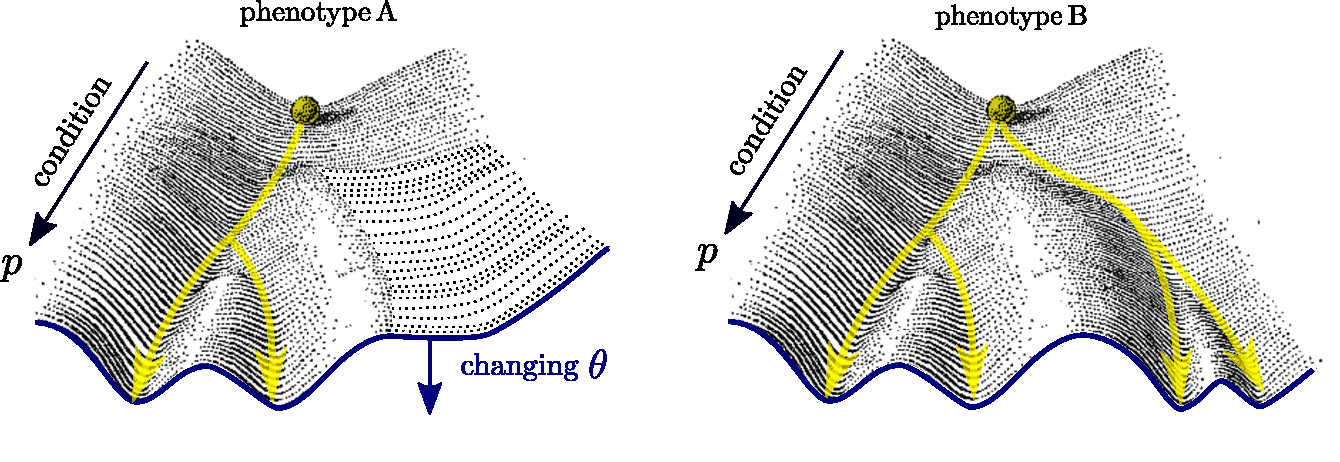
\includegraphics[scale=0.6]{waddington}
\caption{Waddington landscapes representing the set of available behaviours for two phenotypes in response to a controlled condition $p$. Phenotypes are related by changes in landscape topology via changes in $\theta$}
\label{fig:waddington}
\end{Figure}

\noindent
Changing the parameters $\theta$ changes the topology of the valleys potentially giving rise to new behaviours and therefore new phenotypes. Due to the robustness \cite{} and fragility \cite{} of organisms we expect most changes in $\theta$ to either kill the organism or do nothing at all. The emerging picture suggests that the route between phenotypes is a carefully created sequence of changes in $\theta$.

The problem is that the space of decisions that change $\theta$ is intractably large. Furthermore there is no guarantee that any two phenotypes would be connected via experimentally accessible changes in $\theta$. We will see in the incorporated publication in Chapter \ref{chapter:double-exclusive} how differential equation modelling and machine learning can be used to guide experiments and the genetic engineering of \emph{E. coli} towards a phenotype referred to as the \emph{double exclusive reporter}. 

In the collaboration, bifurcation theory \cite{} was used to detect the onset of the desired phenotypic behaviour in a set of differential equations that model the engineered genetic circuits in \emph{E. coli}. We will see in the following sections how bifurcation theory is perfectly suited for modelling transitions between phenotypes, and hence popularised in fields such as synthetic biology and ecology. Through the use of machine learning and bifurcation theory in the same collaboration, we identified a gap: \emph{there existed no differentiable machine learning method that leveraged bifurcation theory directly}. The incorporated publication in Chapter \ref{chapter:inference} fills this gap, enabling an efficient exploration of phenotypes in the high-dimensional space of $\theta$.

\subsection{Differential Equation Models}

In order to leverage bifurcation theory we must describe our organism as a dynamical system. This means that there must be some state $u(t)$, that fully ....

In practice we can only observe a subset of the states, for example by incorporating fluorescent proteins downstream of the coding sequences of the proteins that participate in the antimicrobial resistance. Incorporating any fluorescent proteins into the host genome contributes to cell burdon and at worst can disrupt the mechanism under study. Therefore incorporation sites much be chosen sparsely such that the qualitative behaviour is still observable in the data.

Partial observation can be modelled explicitly with latent variables \cite{} or the explicit modelling of system and measurement device as is done in control theory \cite{}. For the scope of this thesis we will let the modeller have complete freedom on how to choose relevant state variables $u\in\Reals^N$ and write down their own set of differential equations, with unknown parameters $\theta\in\Reals^M$ of the form

\begin{equation}
	\frac{\partial u}{\partial t} = \rates(u)
	\quad\mathrm{where}\quad
	\begin{cases}
		\quad F: \Reals^N\rightarrow\Reals^N \\
		\quad \theta\in\Reals^M
	\end{cases}
	\label{eq:odes}
\end{equation}

\subsection{Microscopic Derivations \& Approximations}
These equations can originate from mean-field approximations of the chemical master equation \cite{} representing biochemical reaction networks \cite{}. This typically yields models with a large number of parameters $M$ and states $N$. The equations could have also undergone a series of quasi-steady state approximations \cite{} yielding hill-functions. Various other model reduction methods exist \cite{} in an attempt to reduce the number of state variables $N$ and parameters $M$.

\subsection{Neural Differential Equations \& Gaussian Processes}
While principled derivation from microscopic rules exist, often the the number of variables $N$ participating in the mechanism under study becomes intractable. When the desire for predictive performance out-weighs the desire for mechanistic explanations, the states $u$ are chosen to be the observable subset for which we have data, and the right-hand side $\rates$ can be a machine learning model such as a neural network or gaussian process \cite{}. In this case the number of parameters becomes much larger than the number of states $M\gg N$. A recent breakthrough in back-propagation through differential equation solvers \cite{} has made these models tractable in optimisation routines, and popularised them in literature \cite{}.

\subsection{Partial Differential Equations}
When studying spatio-temporal dynamics of organisms, a popular choice is to incorporate a diffusive term that models the exchange of matter between spatial locations
\begin{align}
	\partial_t
	\psi &=
	\mathbf{\Gamma}\omega(\psi|\mathbf{\Gamma})
	\label{eq:reaction}
\end{align}

\subsection{Stochastic Differential Equations}

\subsection{Bifurcation Analysis}
In the mean field approximation \eqref{eq:reaction} we may investigate the
steady state $\partial_t\psi=0$. This gives rise to a set of $S$ polynomial
equations in the components $\psi[s]\in[0,\infty)$ of steady state $\psi^*$
These define $S-1$ dimensional nullcline hypersurfaces embedded in $S$
dimensional state-space.
\begin{align}
	\sum_{r=1}^R\Gamma[s',r]\sigma[r]
		\prod_{s=1}^S{\psi[s] \choose g[s,r]}
		\bigg|_{\psi=\psi^*}
		=0\qquad\forall s'=1,2,\dots,S
	\label{eq:steadystate}
\end{align}

\begin{Figure}
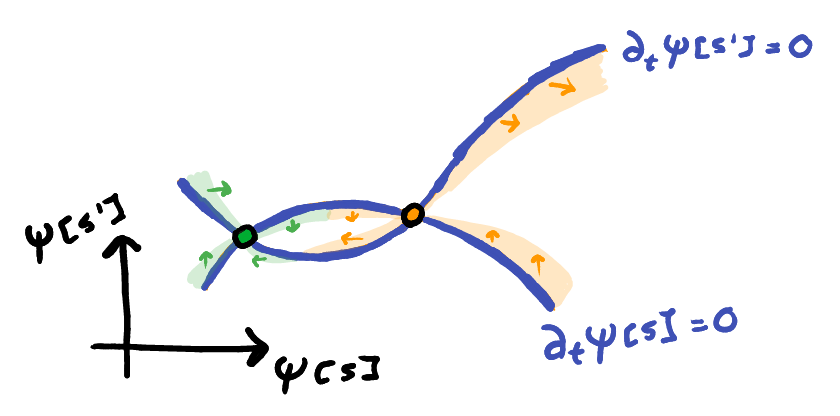
\includegraphics[scale=0.35]{figures/nullclines}
\caption{Schematic of two nullclines with their orthogonal local\\ field flows intersecting
at \textcolor{Green}{stable} and \textcolor{orange}{unstable} fixed points $\psi^*$}
\label{fig:nullclines}
\end{Figure}
Nullclines determine local direction of evolution of the system. On a given
nullcline $\partial_t\psi[s]=0$ the flow of the field must be orthogonal to
the direction of $\psi[s]$. At intersections between two nullclines, the flow
must be orthogonal to the plane defined by two axes. At the interactions between
all nullcline we may find the fixed points $\psi^*$ as shown in Figure \ref{fig:nullclines}.

Classification of fixed points $\psi^*$ is done by linearising the equation of motion
\eqref{eq:reaction} with respect to field perturbation $\varepsilon(t)$ in their vicinity
and determining the eigenvalues of the resultant $S\times S$ Jacobian $\mathbf{J}(\psi)$
evaluated at each fixed point $\psi^*$.
\begin{align}
	\varepsilon(t) \sim
	\mathbb{e}^{\mathbf{J}(\psi)|_{\psi=\psi^*}t}\qquad\qquad\qquad\qquad\qquad\qquad
	\\
	\quad\text{where}\quad
	\mathrm{J}[i,j]=
	\sum_{r=1}^R
	\sigma[r]
\bigg(H(\psi[i])-H(\psi[i]-g[i,r])\bigg)
	\Gamma[j,r]
		\prod_{s=1}^S{\psi[s] \choose g[s,r]}
	\\
	H(x)=\int_0^1\frac{1-t^x}{1-t}\mathrm{d}t\quad
	\text{are generalised Harmonic Numbers}\qquad
	\label{eq:linearstability}
\end{align}
For reactions involving one or two distinguishable particles as
in \eqref{eq:simplifiedpropensity} the nullclines become hyperplanes and the Jacobian
simplifies. We can see that both the reaction topology given by stoichiometric
coefficients $\Gamma[i,j]$ and the reaction rates $\sigma[r]$ contribute to
rotating and shifting the hyperplanes and determining the location and stability
of their intersections.
\begin{align}
	\mathrm{J}[i,j]=
	\sum_{r=1}^R
		\sigma[r]|\Gamma[i,r]|\Gamma[j,r]
		\prod_{\,s\neq i}
		\psi[s]^{g[i,r]}
		\qquad g[i,r]\in\{0,1\} \quad\forall i,r
	\label{eq:simplifiedjacobian}
\end{align}
The sign of eigenvalues $\lambda$ of Jacobian $\mathbf{J}$ determine whether a fixed point
is stable $\lambda<0$ or unstable $\lambda>0$. As an illustrative example we can characterise
fixed points given an arbitrary two dimensional Jacobian. Figure \ref{fig:stability} reveals
the regions of stability and phase space flows.
\begin{Figure}
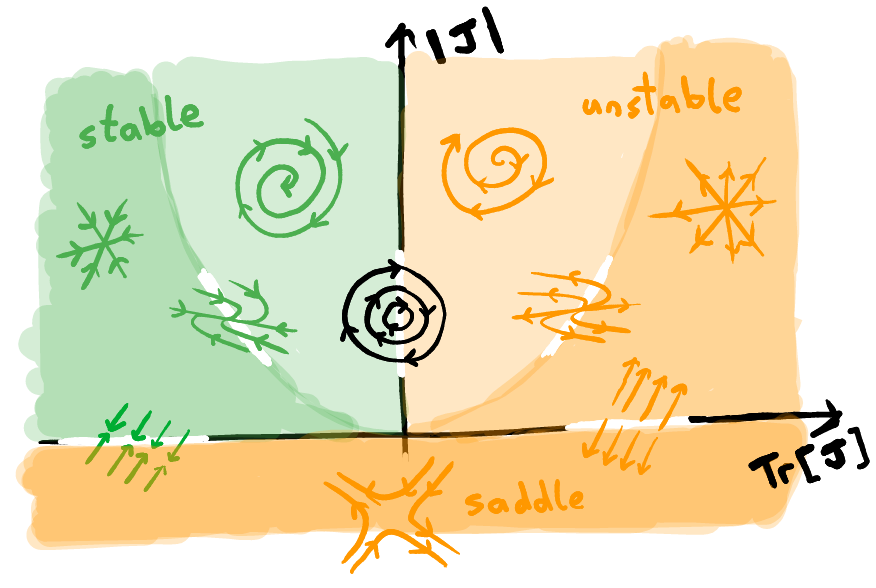
\includegraphics[scale=0.35]{figures/stability}
\caption{Classification of \textcolor{Green}{stable} and \textcolor{orange}{unstable}
fixed points for a general \\two dimensional Jacobian in terms of trace $\mathrm{Tr}[\mathbf{J}]$ and
determinant $|\mathbf{J}|$}
\label{fig:stability}
\end{Figure}

Varying the continuos parameters $\sigma[r]$ moves the nullclines and may result in
the creation or annihilation of fixed points of different classes. While an individual
fixed point may change location and local phase space flow, it cannot change class
without involving another fixed point.

These are called bifurcations and also fall into various categories.
Figure \ref{fig:bifurcations} illustrates some of the possible one parameter
supercritical bifurcations; subcritical cases are obtained by permuting
stabilities of fixed points. Note the hysteresis loop in the saddle-node
bifurcation.
\begin{Figure}
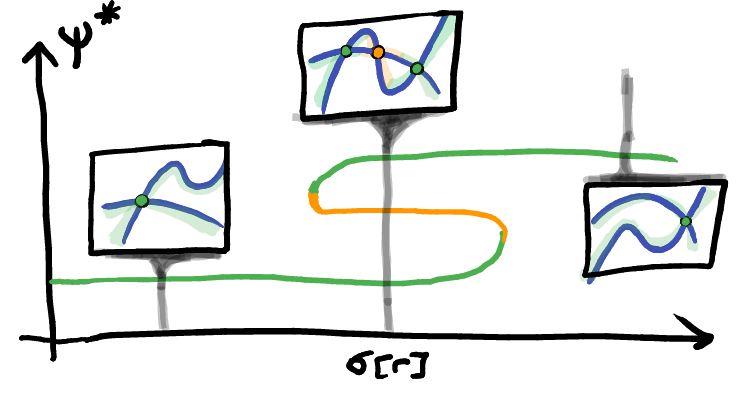
\includegraphics[scale=0.35]{figures/saddlenode}
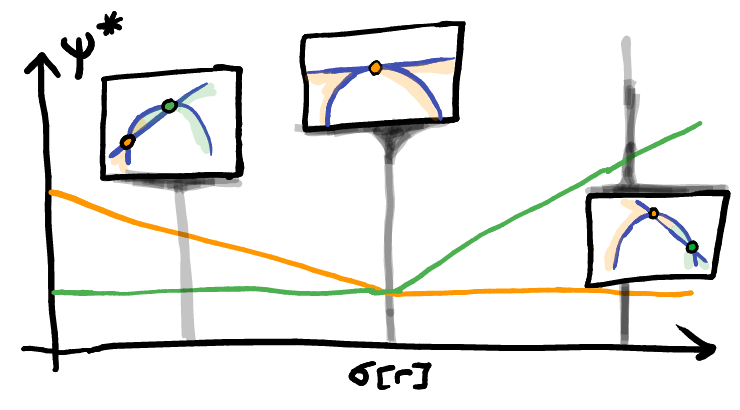
\includegraphics[scale=0.35]{figures/transcritical}
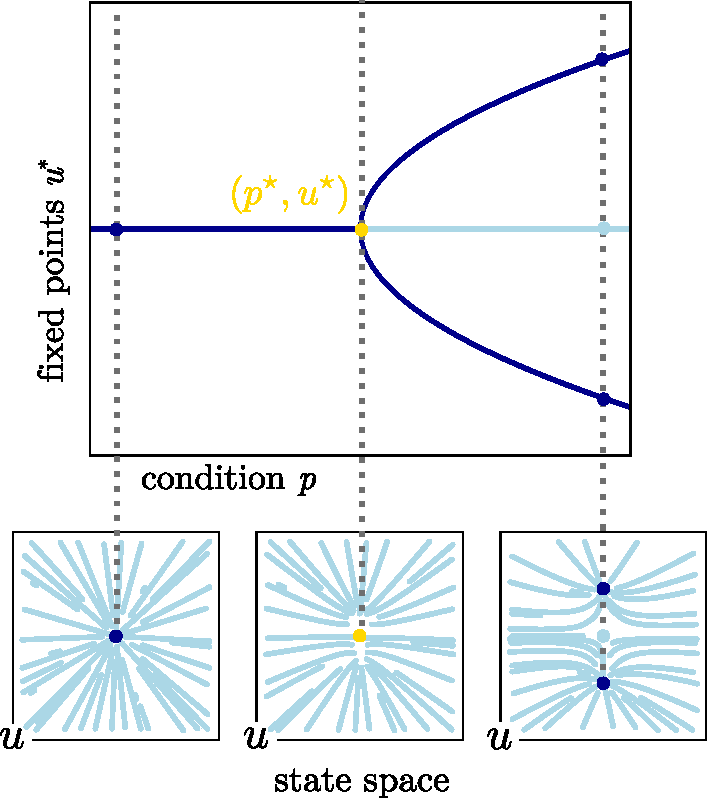
\includegraphics[scale=0.35]{figures/pitchfork}
\caption{Saddle-node, Transcritical and Pitchfork bifurcation diagram showing
\textcolor{Green}{stable} and \\\textcolor{orange}{unstable} fixed points $\psi^*$
as a function of parameter $\sigma[r]$. Insets show nullcline intersections.}
\label{fig:bifurcations}
\end{Figure}

Another category of bifurcations involves limit cycles, which emerge from fixed
points where the linearised Jacobian eigenvalues have no real part. Limit cycles
have circulating field flow as shown in Figure \ref{fig:stability} along the
$\mathrm{Tr}[\mathbf{J}]=0$, $|\mathbf{J}|>0$ axis.

Note how oscillations emerge at small amplitudes in the Hopf bifurcation,
whereas the large amplitude oscillations may instantly emerge in an infinite-period
or cyclic-fold bifurcation. In Figure \ref{fig:limitcycles} the shaded regions
represent the peaks and troughs of the oscillations.
\begin{Figure}
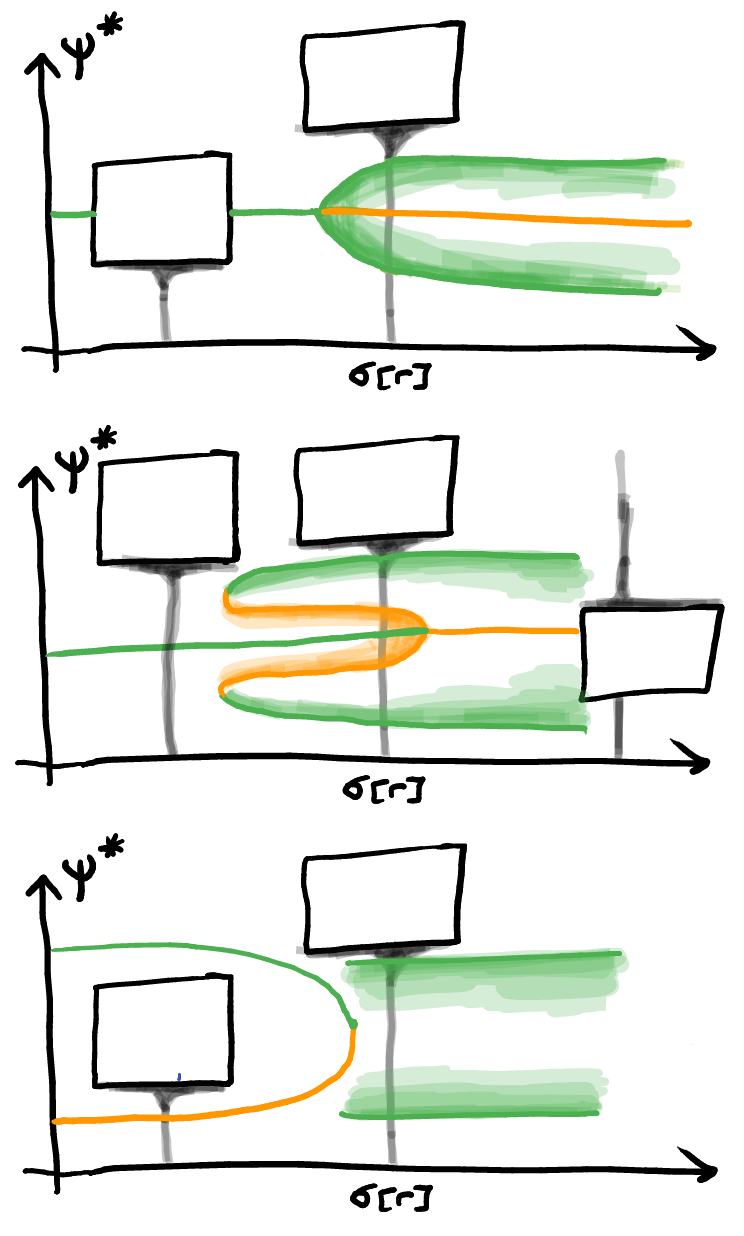
\includegraphics[scale=0.35]{figures/limitcycles}
\caption{Hopf, Cyclic-fold and Infinite-Period bifurcation diagram showing
\textcolor{Green}{stable} and \textcolor{orange}{unstable}\\ fixed points
and limit cycles as a function of parameter $\sigma[r]$.
Insets show nullclines [tbc]}
\label{fig:limitcycles}
\end{Figure}

\subsection{Attractor Geometry and Universality}
In this section we would explore the geometrisation of phase space, lyapunov
exponents and universality. Perhaps a discussion on phase transitions and
the relation to Landau-Ginzberg approaches is required.
Maybe also periodic orbit theory? Depends how useful it is.
\subsection{Reaction-Diffusion}
Here we first introduce diffusion macroscopically by simply adding the laplacian
to mean field equation $\eqref{eq:reaction}$. We introduce the turning bifurcation and
show how linear stability analysis is insufficient to capture pattern formation
and rich inhomogeneous steady states. A promising approach may be geometrisation
of the moving local equilibria \cite{Halatek2018}.

\section{Phenotype Inference with Machine Learning}
\begin{itemize}
    \item Preface on SciML community and gray-box modelling
\end{itemize}

\subsection{Classification and Regression}
\begin{itemize}
    \item Logistic regression
    \item Nearest neighbour methods
    \item Mixture Models
\end{itemize}

\subsection{Dimensionality Reduction Methods}
\begin{itemize}
    \item UMAP and Tsne
    \item Sloppy parameters and identify-ability
\end{itemize}

\subsection{Clustering Methods}
